% FUNDAMENTACAO TEORICA------------------------------------------------------------------

\chapter{FUNDAMENTAÇÃO TEÓRICA}
\label{chap:fundamentacao-teorica}Este capítulo tem por finalidade a apresentação dos aspéctos teóricos e trabalhos relacionados, sendo constituído pelas seguintes seções: Seção 

\section{PLATAFORMA ARDUINO}
\label{sec:arduino} O arduino é uma plataforma de prototipagem eletrônica open-source criada em 2005, que baseia-se em hardware e software flexíveis e de fácil uso, tornando-se acessível para novatos e profissionais. O arduino é capaz de sentir o estado do ambiente através de sensores e interagir com o mesmo por meio de motores e outros atuadores, isto pode ser feito enviando um conjunto de instruções para o microcontrolador através da linguagem de programação Arduino e a IDE Arduino. Por ser uma plataforma open-source, possui uma vasta quantia de contribuições da comunidade mundial, composta por estudantes, programadores, artistas e profissionais, o que gera uma grande quantidade de conhecimento acessível, útil para usuários novatos e experientes \cite{arduino2018}.

Professores e alunos o utilizam a plataforma para o desenvolvimento de instrumentos científicos de baixo custo, ou para introduzir a programação e robótica, além de ser utilizada também por amadores, principalmente pelas seguintes características: baixo custo, as placas são mais baratas em comparação com outros microcontroladores. Multiplataforma, a IDE utilizada para o desenvolvimento de um sketch(nome dado aos programas, uma unidade de código que é carregada e executada em uma placa), chamada de Arduino Software, ´pode ser utilizada em sistemas operacionais Windows, Linux e Mac Os, diferenciando-se dos demais, limitados ao sistema operacional Windows. Ambiente de programação fácil e transparente, o Arduino Software é de fácil utilização e adaptável o suficiente para que usuários avançados tirem um melhor proveito da plataforma. Software open source e flexível, o software Arduino é uma ferramenta open source, podendo ser modificada e aprimorada por usuários experientes. A linguagem pode ser expandida através de bibliotecas em C++, além disto, pode-se adicionar trechos de código da linguagem de programação AVR-C nos programas do Arduino. Hardware open source e flexível, os planos das placas Arduino são publicados sob uma licena Creative Commons, permitindo o aprimoramento e criação de novos módulos.\cite{arduino2018}

\section{TESTE DE SOFTWARE}
\label{sec:testeDeSoftware} A computação evoluiu muito nas últimas décadas, sendo utilizada em diversas áreas da atividade humana, demandando qualidade e produtividade, e a engenharia de software acompanhou esse progresso, estabelecendo técnicas, critérios, métodos e ferramentas para o desenvolvimento de programas. A engenharia de software pode ser definida como uma disciplina que aplica os princípios da engenharia para a produção de softwares de alta qualidade e baixo custo\cite{Pressman1997}. Apesar dos métodos e técnicas empregadas na produção de softwares, ainda podem ocorrer erros no produto, e com o intuito de minimizar a ocorrência destes, algumas atividades são introduzidas ao longo de todo o processo de desenvolvimento, sendo o teste de software a mais utilizada \cite{Maldonado1997}, constituindo-se em um dos elementos para oferecer evidencias da confiabilidade do software.

Os testes de softwares são compostos por quatro etapas: planejamento de testes, projeto de caso de testes, execução e avaliação dos resultados dos testes, que são executadas ao longo do desenvolvimento do software e efetivam-se em três diferentes fases de teste: de unidade, de integração e de sistema. Onde o primeiro, dedica-se na menor unidade do projeto, identificando erros de lógica e implementação em cada parte do programa. O teste de integração é realizado durante a integração da estrutura do programa, e tem como objetivo, a partir dos módulos testados no nível de unidade, construir a estrutura do programa, na forma determinada pelo projeto. O teste de sistema, é realizado após a integração do sistema, identificando erros de funções e características de desempenho que não estejam na especificação.\cite{Maldonado2004}

\begin{figure}[!htb]
    \centering
    \caption{Modelo das etapas do teste de software}
    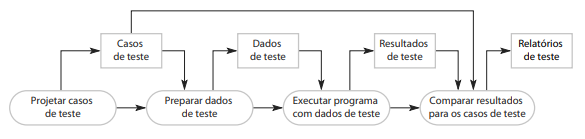
\includegraphics[width=1\textwidth]{./dados/figuras/Modelo_processo_de_software}
    \fonte{\cite{iansommerville}}
    \label{fig:figura-modelo-etapas-teste-de-software}
\end{figure}

As práticas pertinentes ao teste do software não abrangem somente a execução do programa, denominado teste dinâmico, existem também os testes estáticos, que não necessitam da execução de um software para serem realizados, podendo aplicá-los em diferentes artefatos como a revisão de documentos de requisitos e análise do código fonte.\cite{Pedro}

Os teste funcionais, conhecido como teste de caixa-preta e os testes estruturais, também chamados de teste de caixa-branca, são exemplos de técnicas de teste de software. No primeiro, não há a necessidade do testador conhecer a codificação, ele apenas informa os dados de entrada e examina se a saída está de acordo com o esperado, portanto os testes de caixa-preta visam detectar se o sistema aceita entradas incorretas, se a saída gerada está correta, se existem erros na interface e a falta de alguma funcionalidade. O segundo, observa a estrutura do código fonte para identificar a implementação e se os testes estão cobrindo diferentes caminhos, sendo assim, estes testes são implementados de forma a testar decisões logicas, variáveis estáticas, variáveis dinâmicas e \textit{loops}, por exemplo.\cite{Pedro}


\section{MANUTENÇÃO DE SOFTWARE}
\label{sec:manutencaoDeSoftware}

A vida de um sistema de computação não é finalizada após a sua implementação, ele ainda será utilizado por muito tempo, e com certeza passará por muitas atualizações, tanto para correção de erros ou apenas para otimização. Uma das fases do processo de desenvolvimento de software é a manutenção de software, este é um procedimento de melhoria de um programa que já foi desenvolvido, ou seja, já está em ambiente de produção, ou que ainda está em desenvolvimento. Com a manutenção também é realizado a correção dos erros encontrados por usuários do sistema ou testes realizados por desenvolvedores \cite{rodrigoSpinola2011}.

Existem diversas razões para que um software sofra alterações, principalmente se este implementar soluções aproximadas para problemas do mundo real, por exemplo, com o passar do tempo, conforme o melhor entendimento do problema, pode-se encontrar uma melhor solução, ou ainda, alterações de legislações de um determinado país ou novos requisitos do cliente.

A manutenção de software pode ser dividida em diferentes tipos, segundo \cite{Pressman2005} é dividida em 4 tipos:


\begin{itemize}
    \item \textbf{Manutenção Corretiva:} Correção de erros que não foram detectados na fase de teste, que podem não atrapalhar o funcionamento do software, sendo corrigidos por simples reparações, ou defeitos mais complexos, que exijam uma manutenção temporária, com o objetivo de manter o funcionamento normal do software e posteriormente disponibilizar uma correção definitiva em uma nova versão. 
\end{itemize}
    
\begin{itemize}  
    \item \textbf{Manutenção Adaptativa:} Adequação do software em relação as mudanças ocorridas no ambiente externo, que podem ser mudanças na regra de negócio, novos sistemas operacionais que não sejam compatível com o software, nova plataforma de hardware ou mudanças na constituição e leis que afetam funções do sistema.
\end{itemize}
    
 \begin{itemize}  
    \item Manutenção Evolutiva (ou perfectiva):
\end{itemize}
    
\begin{itemize}  
    \item Manutenção Preventiva (reegenharia):
\end{itemize}
    








\section{PROCESSO DE SOFTWARE}
\label{sec:processoDeSoftware}